\documentclass[aspectratio=169]{../latex_main/tntbeamer}


\usepackage{dsfont}
\usepackage{bm}
\usepackage[english]{babel}
\usepackage[T1]{fontenc}
%\usepackage[utf8]{inputenc}
\usepackage{graphicx}
\graphicspath{ {./figures/} }
\usepackage{algorithm}
\usepackage[ruled,vlined,algo2e,linesnumbered]{algorithm2e}
\usepackage{hyperref}
\usepackage{booktabs}
\usepackage{mathtools}

\usepackage{amsmath,amssymb}

\DeclareMathOperator*{\argmax}{arg\,max}
\DeclareMathOperator*{\argmin}{arg\,min}

\usepackage{pgfplots}
\pgfplotsset{compat=1.16}
\usepackage{tikz}
\usetikzlibrary{trees} 
\usetikzlibrary{shapes.geometric}
\usetikzlibrary{positioning,shapes,shadows,arrows,calc,mindmap}
\usetikzlibrary{positioning,fadings,through}
\usetikzlibrary{decorations.pathreplacing}
\usetikzlibrary{intersections}
\pgfdeclarelayer{background}
\pgfdeclarelayer{foreground}
\pgfsetlayers{background,main,foreground}
\tikzstyle{activity}=[rectangle, draw=black, rounded corners, text centered, text width=8em]
\tikzstyle{data}=[rectangle, draw=black, text centered, text width=8em]
\tikzstyle{myarrow}=[->, thick, draw=black]

% Define the layers to draw the diagram
\pgfdeclarelayer{background}
\pgfdeclarelayer{foreground}
\pgfsetlayers{background,main,foreground}

% Requires XeLaTeX or LuaLaTeX
\usepackage{unicode-math}

\usepackage{fontspec}
%\setsansfont{Arial}
\setsansfont{RotisSansSerifStd}[ 
Path=../latex_main/fonts/,
Extension = .otf,
UprightFont = *-Regular,  % or *-Light
BoldFont = *-ExtraBold,  % or *-Bold
ItalicFont = *-Italic
]
\setmonofont{Cascadia Mono}[
Scale=0.8
]

% scale factor adapted; mathrm font added (Benjamin Spitschan @TNT, 2021-06-01)
%\setmathfont[Scale=1.05]{Libertinus Math}
%\setmathrm[Scale=1.05]{Libertinus Math}

% other available math fonts are (not exhaustive)
% Latin Modern Math
% XITS Math
% Libertinus Math
% Asana Math
% Fira Math
% TeX Gyre Pagella Math
% TeX Gyre Bonum Math
% TeX Gyre Schola Math
% TeX Gyre Termes Math

% Literature References
\newcommand{\lit}[2]{\href{#2}{\footnotesize\color{black!60}[#1]}}

%%% Beamer Customization
%----------------------------------------------------------------------
% (Don't) Show sections in frame header. Options: 'sections', 'sections light', empty
\setbeamertemplate{headline}{empty}

% Add header logo for normal frames
\setheaderimage{
	% 
\includegraphics[height=\logoheight]{figures/TNT_darkv4.pdf}
	
\includegraphics[height=\logoheight]{../latex_main/figures/luh_logo_rgb_0_80_155.pdf}
	% 
\includegraphics[height=\logoheight]{figures/logo_tntluh.pdf}
}

% Header logo for title page
\settitleheaderimage{
	% 
\includegraphics[height=\logoheight]{figures/TNT_darkv4.pdf}
	
\includegraphics[height=\logoheight]{../latex_main/figures/luh_logo_rgb_0_80_155.pdf}
	% 
\includegraphics[height=\logoheight]{figures/logo_tntluh.pdf}
}

% Title page: tntdefault 
\setbeamertemplate{title page}[tntdefault]  % or luhstyle
% Add optional title image here
%\addtitlepageimagedefault{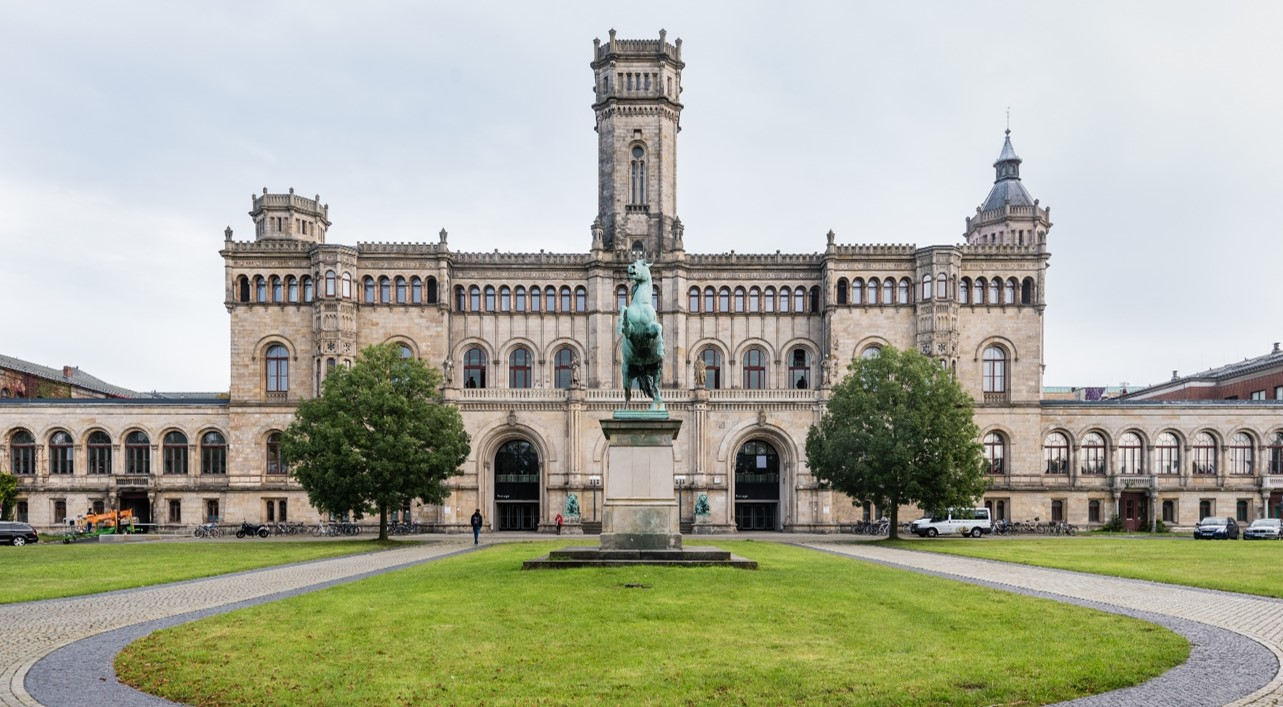
\includegraphics[width=0.65\textwidth]{figures/luh_default_presentation_title_image.jpg}}

% Title page: luhstyle
% \setbeamertemplate{title page}[luhstyle]
% % Add optional title image here
% \addtitlepageimage{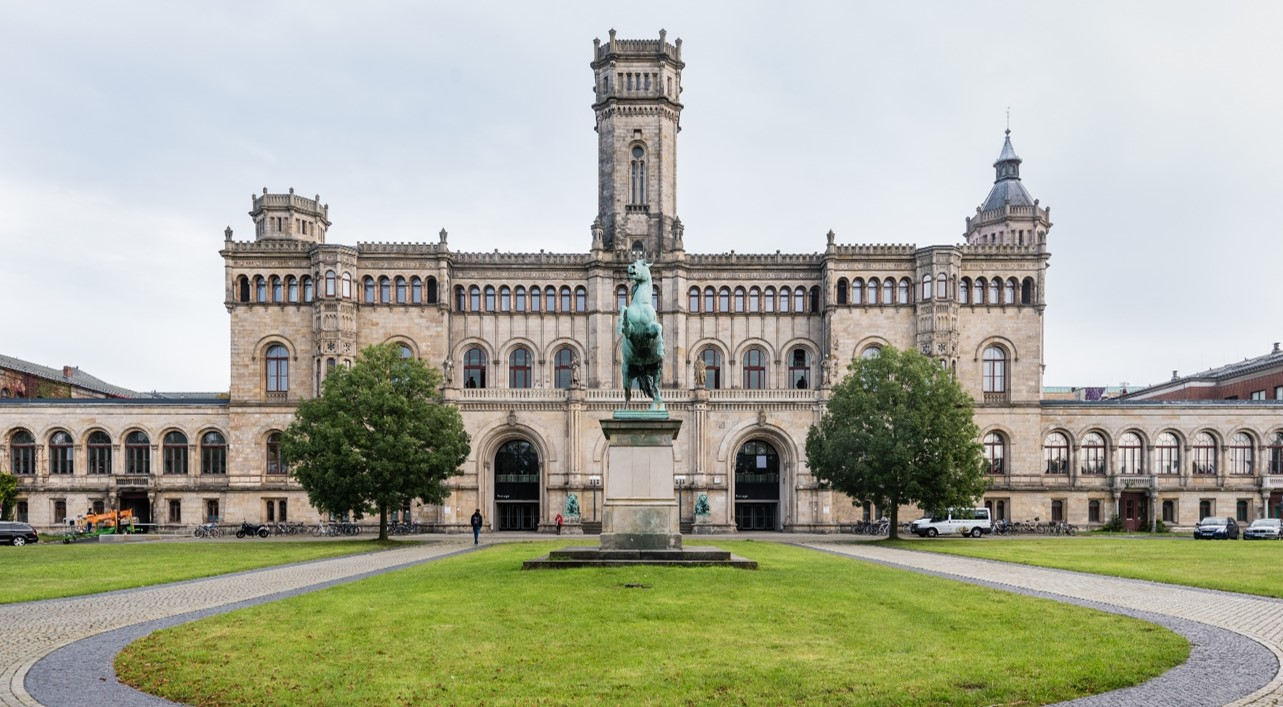
\includegraphics[width=0.75\textwidth]{figures/luh_default_presentation_title_image.jpg}}

\author[Lindauer \& Anand]{Marius Lindauer and Avishek Anand\\[1em]
	
\includegraphics[height=\logoheight]{../latex_main/figures/luh_logo_rgb_0_80_155.pdf}\qquad

\includegraphics[height=\logoheight]{../latex_main/figures/TNT_darkv4}\qquad

\includegraphics[height=\logoheight]{../latex_main/figures/L3S.jpg}	}
\date{Winter Term 2021
}


%%% Custom Packages
%----------------------------------------------------------------------
% Create dummy content
\usepackage{blindtext}

% Adds a frame with the current page layout. Just call \layout inside of a frame.
\usepackage{layout}


\title{iML: Post-hoc Methods for Neural Networks}
\subtitle{Motivation}
\begin{document}
	\maketitle
	\graphicspath{ {./figure/} }
	
\begin{frame}[c]{Neural Networks as Complex ML models}
	\pause
	\begin{itemize}
		\item Neural networks are over parameterised
		\begin{itemize}
			\item Vision models and Language models routinely have > millions of params
			\item Sometimes \#parameters > \#input instances
			\item Which and how do the features, parameters, training instances contribute towards
				  the final decision ?
		\end{itemize}
	\end{itemize}
	\pause
	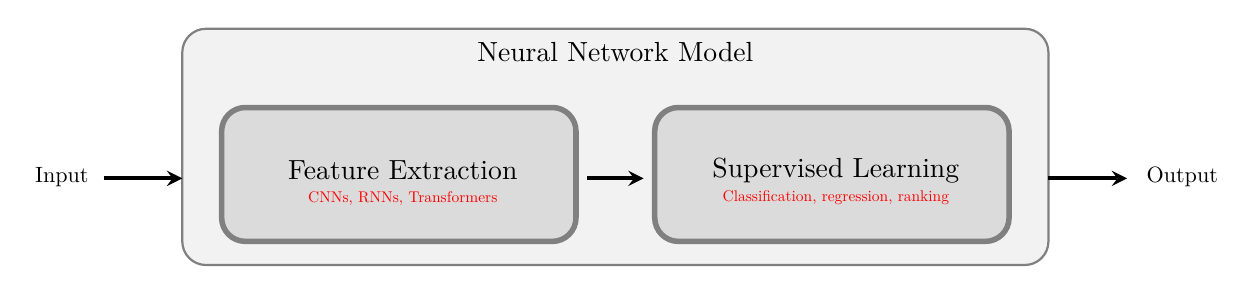
\begin{tikzpicture}
		\filldraw[color=gray, fill=gray!10, rounded corners= 3mm, thick]  (-1,0) rectangle (10,-3); 
		\node at (4.5, -0.3) {Neural Network Model}; 
		\filldraw[color=gray, fill= gray!28, rounded corners= 3mm, line width= 0.7mm] (-0.5, -1) rectangle (4, 					-2.7);
		\node  at (1.8, -1.8) {Feature Extraction};
		\node [color=red, scale=0.56] at (1.8, -2.15) {CNNs, RNNs, Transformers};
		\draw [-stealth,line width = .5mm, scale= 2] (-1, -0.95) -- (-0.50, -0.95);
		\node [scale= 0.8] at (-2.53, -1.88) {Input};
		\draw [-stealth,line width = .5mm, scale= 2] (5, -0.95) -- (5.50, -0.95);
		\draw [-stealth,line width = .5mm, scale= 2] (2.07, -0.95) -- (2.43, -0.95);
		\filldraw[color=gray, fill= gray!28, rounded corners= 3mm, line width= 0.7mm] (5, -1) rectangle (9.5, -2.7);
		\node [scale= 0.8] at (11.7, -1.88) {Output};
		\node [color=red, scale=0.56] at (7.3, -2.15) {Classification, regression, ranking};
		\node at (7.3, -1.8) {Supervised Learning};
\end{tikzpicture}
\end{frame}


\begin{frame}{Neural Networks as Complex ML models}
	\begin{itemize}
		\item Neural networks are compositional and non-linear systems
		\begin{itemize}
			\item The success of neural networks is due to their depth
			\begin{itemize}
				\item Depth results in compositional behaviour
			\end{itemize}
			\item Non-linearity between layers helps capture non-linear relationships
		\end{itemize}
		\bigskip
		
		\item Depth and non-linearity leads to lack of interpretability
	\end{itemize}

    \hfill
    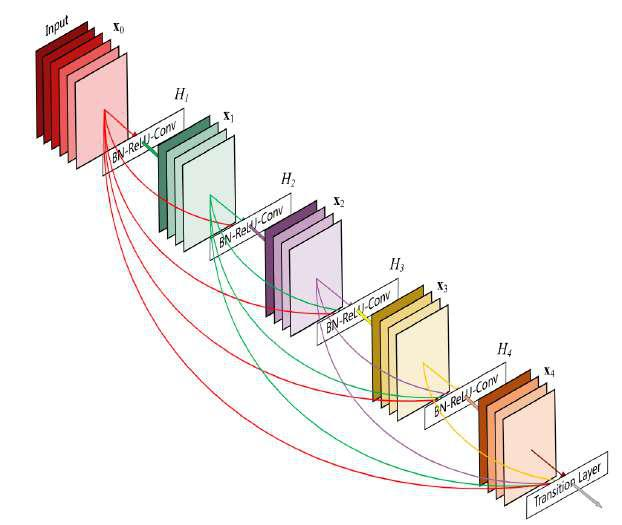
\includegraphics[scale=.4]{img116}

\end{frame}

\begin{frame}[c]{Model-specific interpretability}
	\begin{itemize}
		\item What types of neural models are out there ?
		\begin{itemize}
			\item For vision: Convolutional Neural Nets
			\item For language, speech: Recurrent Neural Nets, Transformer Models
			\item For recommendation systems, ranking: Factorization-based Models, Embeddings
models
		\end{itemize}
		\item Each of the domains have their challenges and have developed specific approaches for
interpretability
		\begin{itemize}
			\item We will focus on first principles that can be applied to most models
			\item We will discuss adaptations to each data modality as and when required
		\end{itemize}
	\end{itemize}
	
\end{frame}

% \begin{frame}[c]{Interpretability landscape in Neural Networks}
%     \begin{tikzpicture}
% 	\filldraw[color=gray, fill=gray!28, rounded corners= 3mm, very thick]  (-1,0) rectangle (6,-1); 
% 	\node at (2.5, -0.5) {Interpretability}; 
% 	\filldraw[color=gray, fill= gray!28, rounded corners= 3mm, very thick] (-2.8, -3) rectangle (0, -4.0);

% 	\node  [scale=.7] at (-1.4, -3.4) {Interpretability by 
% };
% 	\node  [scale=.7] at (-1.5, -3.7) {desgin
% };
% 	\node [color=red, scale=0.56] at (2.4, -1.35) {During vs after training};
% 	\draw [-stealth,line width = .5mm, scale= 2] (0, -0.5) -- (-0.70, -1.5);
% 	%\node [scale= 0.8] at (-2.53, -1.88) {Input};
% 	\draw [-stealth,line width = .5mm, scale= 2] (2.5, -0.5) -- (3.50, -1.5);
% 	%\draw [-stealth,line width = .5mm, scale= 2] (2.07, -0.95) -- (2.43, -0.95);
% 	\filldraw[color=gray, fill= gray!28, rounded corners= 3mm, very thick] (5.8, -3) rectangle (9, -4.0);
% 	%\node [scale= 0.8] at (11.7, -1.88) {Output};
% 	%\node [color=red, scale=0.56] at (7.3, -2.15) {Classification, regression, ranking};
% 	\node [scale=.8] at (7.3, -3.3) {Post-hoc};
% 	\node [scale=.8] at (7.4, -3.65) {Interpretability};
% 	\end{tikzpicture}
% \end{frame}

% \begin{frame}[c]{Interpretability landscape in Neural Networks}
%     \begin{tikzpicture}
% 	\filldraw[color=gray, fill=gray!28, rounded corners= 3mm, very thick]  (-1,0) rectangle (6,-1); 
% 	\node at (2.5, -0.5) {Interpretability}; 
% 	\filldraw[color=gray, fill= gray!28, rounded corners= 3mm, very thick] (-2.8, -3) rectangle (0, -4.0);
% 	\node  [scale=.7] at (-1.4, -3.4) {Interpretability by 
% };
% 	\node  [scale=.7] at (-1.5, -3.7) {desgin
% };
% 	\node [color=red, scale=0.56] at (2.4, -1.35) {During vs after training};
% 	\draw [-stealth,line width = .5mm, scale= 2] (0, -0.5) -- (-0.70, -1.5);
% 	%\node [scale= 0.8] at (-2.53, -1.88) {Input};
% 	\draw [-stealth,line width = .5mm, scale= 2] (2.5, -0.5) -- (3.50, -1.5);
% 	%\draw [-stealth,line width = .5mm, scale= 2] (2.07, -0.95) -- (2.43, -0.95);
% 	\filldraw[color=gray, fill= gray!28, rounded corners= 3mm, very thick] (5.8, -3) rectangle (9, -4.0);
% 	%\node [scale= 0.8] at (11.7, -1.88) {Output};
% 	%\node [color=red, scale=0.56] at (7.3, -2.15) {Classification, regression, ranking};
% 	\node [scale=.8] at (7.3, -3.3) {Post-hoc};
% 	\node [scale=.8] at (7.4, -3.65) {Interpretability};
	
% 	\filldraw[color=gray, fill= gray!28, rounded corners= 3mm, very thick] (7.5, -5) rectangle (10.1, -6.0);
% 	\filldraw[color=gray, fill= gray!28, rounded corners= 3mm, very thick] (3.8, -5) rectangle (6.1, -6.0);
% 	\draw [-stealth,line width = .5mm, scale= 2] (3, -2) -- (2.3, -2.5);
% 	\draw [-stealth,line width = .5mm, scale= 2] (3.5, -2) -- (4.30, -2.5);
% 	\node [scale=.6] at (4.95, -5.3) {Black-box or Model};
% 	\node [scale=.6] at (4.90, -5.65) {agnostic};
% 	\node [scale=.6] at (8.8, -5.3) {White-box or Model};
% 	\node [scale=.6] at (8.75, -5.65) {introspective};
% 	\node [scale=.6, color=red] at (6.6, -4.5) {Access to params.};
% 	\node [scale=.4, color=blue] at (4.90, -6.1) {No access to model params,};
% 	\node [scale=.4, color=blue] at (4.93, -6.3) {LIME, LORE, SHAP};
% 	\end{tikzpicture}
% \end{frame}

% \begin{frame}[c]{Interpretability landscape in Neural Networks}
%     \begin{tikzpicture}
% 	\filldraw[color=gray, fill=gray!28, rounded corners= 3mm, very thick]  (-1,0) rectangle (6,-1); 
% 	\node at (2.5, -0.5) {Interpretability}; 
% 	\filldraw[color=gray, fill= gray!28, rounded corners= 3mm, very thick] (-2.8, -3) rectangle (0, -4.0);
% 	\node  [scale=.7] at (-1.4, -3.4) {Interpretability by 
% };
% 	\node  [scale=.7] at (-1.5, -3.7) {desgin
% };
% 	\node [color=red, scale=0.56] at (2.4, -1.35) {During vs after training};
% 	\draw [-stealth,line width = .5mm, scale= 2] (0, -0.5) -- (-0.70, -1.5);
% 	%\node [scale= 0.8] at (-2.53, -1.88) {Input};
% 	\draw [-stealth,line width = .5mm, scale= 2] (2.5, -0.5) -- (3.50, -1.5);
% 	%\draw [-stealth,line width = .5mm, scale= 2] (2.07, -0.95) -- (2.43, -0.95);
% 	\filldraw[color=gray, fill= gray!28, rounded corners= 3mm, very thick] (5.8, -3) rectangle (9, -4.0);
% 	%\node [scale= 0.8] at (11.7, -1.88) {Output};
% 	%\node [color=red, scale=0.56] at (7.3, -2.15) {Classification, regression, ranking};
% 	\node [scale=.8] at (7.3, -3.3) {Post-hoc};
% 	\node [scale=.8] at (7.4, -3.65) {Interpretability};
	
% 	\filldraw[color=gray, fill= gray!28, rounded corners= 3mm, very thick] (7.5, -5) rectangle (10.1, -6.0);
% 	\filldraw[color=gray, fill= gray!28, rounded corners= 3mm, very thick] (3.8, -5) rectangle (6.1, -6.0);
% 	\draw [-stealth,line width = .5mm, scale= 2] (3, -2) -- (2.3, -2.5);
% 	\draw [-stealth,line width = .5mm, scale= 2] (3.5, -2) -- (4.30, -2.5);
% 	\node [scale=.6] at (4.95, -5.3) {Black-box or Model};
% 	\node [scale=.6] at (4.90, -5.65) {agnostic};
% 	\node [scale=.6] at (8.8, -5.3) {White-box or Model};
% 	\node [scale=.6] at (8.75, -5.65) {introspective};
% 	\node [scale=.6, color=red] at (6.6, -4.5) {Access to params.};
% 	\node [scale=.4, color=blue] at (4.90, -6.1) {No access to model params,};
% 	\node [scale=.4, color=blue] at (4.93, -6.3) {LIME, LORE, SHAP};	
% 	\draw [-stealth,line width = .5mm, scale= 2] (4.10, -3) -- (3.7, -3.5);
% 	\draw [-stealth,line width = .5mm, scale= 2] (4.70, -3) -- (5.20, -3.5);
% 	\filldraw[color=gray, fill= gray!28, rounded corners= 3mm, very thick] (6, -7) rectangle (8, -8.0);
% 	\filldraw[color=gray, fill= gray!28, rounded corners= 3mm, very thick] (10, -7) rectangle (12.1, -8.0);
% 	\node [scale=.8] at (7, -7.5) {Global};
% 	\node [scale=.8] at (11, -7.5) {Local};
% 	\node [scale=.4, color=blue] at (7, -8.2) {Feature visualisation approaches};
% 	\node [scale=.5, color=red] at (8.85, -6.7) {Instance wise vs global};
% 	\end{tikzpicture}
% \end{frame}

% \begin{frame}[c]{Interpretability landscape in Neural Networks}
%     \begin{tikzpicture}
% 		\filldraw[color=gray, fill=gray!28, rounded corners= 3mm, very thick]  (-1,0) rectangle (6,-1); 
% 	\node at (2.5, -0.5) {Interpretability}; 
% 	\filldraw[color=gray, fill= gray!28, rounded corners= 3mm, very thick] (-2.8, -3) rectangle (0, -4.0);
% 	\node  [scale=.7] at (-1.4, -3.4) {Interpretability by 
% };
% 	\node  [scale=.7] at (-1.5, -3.7) {desgin
% };
% 	\node [color=red, scale=0.56] at (2.4, -1.35) {During vs after training};
% 	\draw [-stealth,line width = .5mm, scale= 2] (0, -0.5) -- (-0.70, -1.5);
% 	%\node [scale= 0.8] at (-2.53, -1.88) {Input};
% 	\draw [-stealth,line width = .5mm, scale= 2] (2.5, -0.5) -- (3.50, -1.5);
% 	%\draw [-stealth,line width = .5mm, scale= 2] (2.07, -0.95) -- (2.43, -0.95);
% 	\filldraw[color=gray, fill= gray!28, rounded corners= 3mm, very thick] (5.8, -3) rectangle (9, -4.0);
% 	%\node [scale= 0.8] at (11.7, -1.88) {Output};
% 	%\node [color=red, scale=0.56] at (7.3, -2.15) {Classification, regression, ranking};
% 	\node [scale=.8] at (7.3, -3.3) {Post-hoc};
% 	\node [scale=.8] at (7.4, -3.65) {Interpretability};
	
% 	\filldraw[color=gray, fill= gray!28, rounded corners= 3mm, very thick] (7.5, -5) rectangle (10.1, -6.0);
% 	\filldraw[color=gray, fill= gray!28, rounded corners= 3mm, very thick] (3.8, -5) rectangle (6.1, -6.0);
% 	\draw [-stealth,line width = .5mm, scale= 2] (3, -2) -- (2.3, -2.5);
% 	\draw [-stealth,line width = .5mm, scale= 2] (3.5, -2) -- (4.30, -2.5);
% 	\node [scale=.6] at (4.95, -5.3) {Black-box or Model};
% 	\node [scale=.6] at (4.90, -5.65) {agnostic};
% 	\node [scale=.6] at (8.8, -5.3) {White-box or Model};
% 	\node [scale=.6] at (8.75, -5.65) {introspective};
% 	\node [scale=.6, color=red] at (6.6, -4.5) {Access to params.};
% 	\node [scale=.4, color=blue] at (4.90, -6.1) {No access to model params,};
% 	\node [scale=.4, color=blue] at (4.93, -6.3) {LIME, LORE, SHAP};	
% 	\draw [-stealth,line width = .5mm, scale= 2] (4.10, -3) -- (3.7, -3.5);
% 	\draw [-stealth,line width = .5mm, scale= 2] (4.70, -3) -- (5.20, -3.5);
% 	\filldraw[color=gray, fill= gray!28, rounded corners= 3mm, very thick] (6, -7) rectangle (8, -8.0);
% 	\filldraw[color=gray, fill= gray!28, rounded corners= 3mm, very thick] (10, -7) rectangle (12.1, -8.0);
% 	\node [scale=.8] at (7, -7.5) {Global};
% 	\node [scale=.8] at (11, -7.5) {Local};
% 	\node [scale=.4, color=blue] at (7, -8.2) {Feature visualisation approaches};
% 	\node [scale=.5, color=red] at (8.85, -6.7) {Instance wise vs global};
	
% 	\filldraw[color=gray, fill= gray!28, rounded corners= 3mm, very thick] (-4, -5) rectangle (-2, -6.0);
% 	\filldraw[color=gray, fill= gray!28, rounded corners= 3mm, very thick] (-0.7, -5) rectangle (1.3, -6.0);
% 	\node [scale=.6] at (-3, -5.5) {Simple Models};
% 	\node [scale=.6] at (0.3, -5.4){Sparsity-based};
% 	\node [scale=.6] at (0.35, -5.7){Models};
% 	\node [scale=.5, color=red] at (-1.5, -4.5) {Model Simplicity};
% 	\draw [-stealth,line width = .5mm, scale= 2] (-1.0, -2) -- (-1.5, -2.5);
% 	\draw [-stealth,line width = .5mm, scale= 2] (-0.5, -2) -- (-0, -2.5);	
% 	\node [scale=.4, color=blue] at (-3.0, -6.2) {GAMs, Decision trees,};
% 	\end{tikzpicture}
% \end{frame}

\begin{frame}[c]{Interpretability landscape in Neural Networks}
    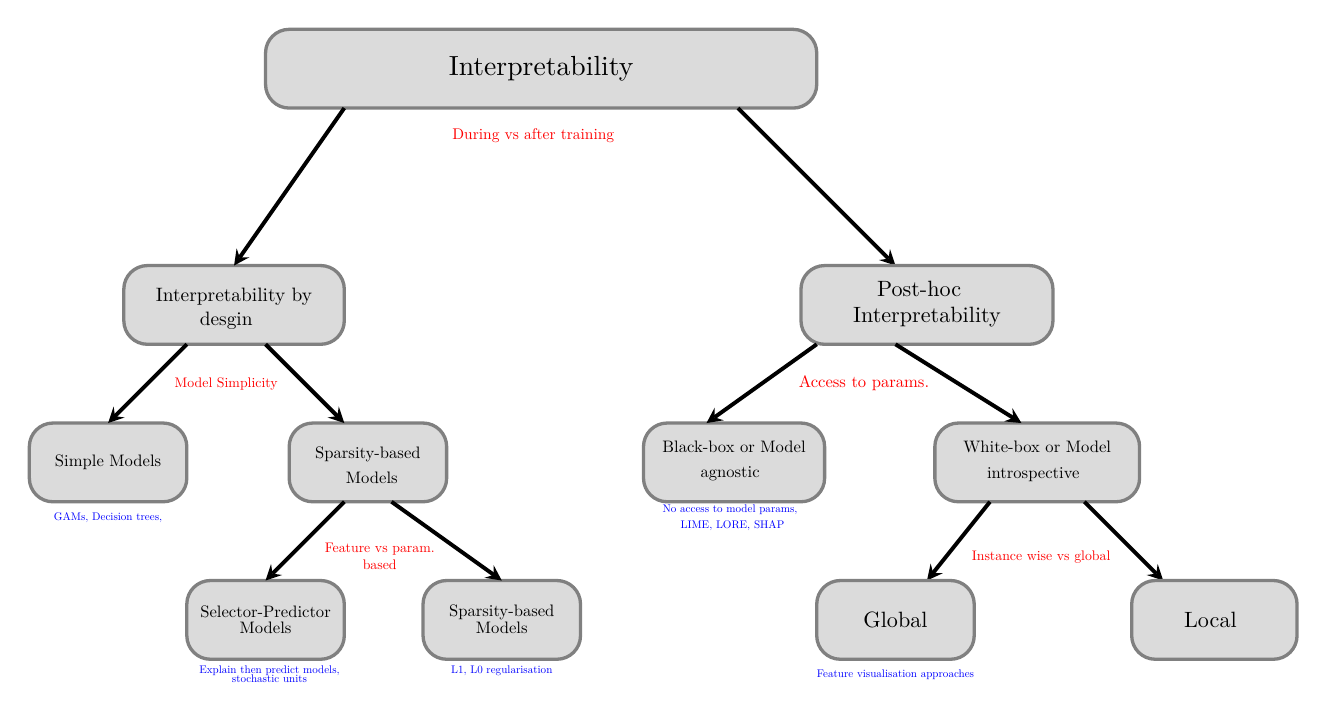
\begin{tikzpicture}
	\filldraw[color=gray, fill=gray!28, rounded corners= 3mm, very thick]  (-1,0) rectangle (6,-1); 
	\node at (2.5, -0.5) {Interpretability}; 
	\filldraw[color=gray, fill= gray!28, rounded corners= 3mm, very thick] (-2.8, -3) rectangle (0, -4.0);
	\node  [scale=.7] at (-1.4, -3.4) {Interpretability by 
};
	\node  [scale=.7] at (-1.5, -3.7) {desgin
};
	\node [color=red, scale=0.56] at (2.4, -1.35) {During vs after training};
	\draw [-stealth,line width = .5mm, scale= 2] (0, -0.5) -- (-0.70, -1.5);
	%\node [scale= 0.8] at (-2.53, -1.88) {Input};
	\draw [-stealth,line width = .5mm, scale= 2] (2.5, -0.5) -- (3.50, -1.5);
	%\draw [-stealth,line width = .5mm, scale= 2] (2.07, -0.95) -- (2.43, -0.95);
	\filldraw[color=gray, fill= gray!28, rounded corners= 3mm, very thick] (5.8, -3) rectangle (9, -4.0);
	%\node [scale= 0.8] at (11.7, -1.88) {Output};
	%\node [color=red, scale=0.56] at (7.3, -2.15) {Classification, regression, ranking};
	\node [scale=.8] at (7.3, -3.3) {Post-hoc};
	\node [scale=.8] at (7.4, -3.65) {Interpretability};
	\pause
	
	\filldraw[color=gray, fill= gray!28, rounded corners= 3mm, very thick] (7.5, -5) rectangle (10.1, -6.0);
	\filldraw[color=gray, fill= gray!28, rounded corners= 3mm, very thick] (3.8, -5) rectangle (6.1, -6.0);
	\draw [-stealth,line width = .5mm, scale= 2] (3, -2) -- (2.3, -2.5);
	\draw [-stealth,line width = .5mm, scale= 2] (3.5, -2) -- (4.30, -2.5);
	\node [scale=.6] at (4.95, -5.3) {Black-box or Model};
	\node [scale=.6] at (4.90, -5.65) {agnostic};
	\node [scale=.6] at (8.8, -5.3) {White-box or Model};
	\node [scale=.6] at (8.75, -5.65) {introspective};
	\node [scale=.6, color=red] at (6.6, -4.5) {Access to params.};
	\node [scale=.4, color=blue] at (4.90, -6.1) {No access to model params,};
	\node [scale=.4, color=blue] at (4.93, -6.3) {LIME, LORE, SHAP};
	\pause
	
	\draw [-stealth,line width = .5mm, scale= 2] (4.10, -3) -- (3.7, -3.5);
	\draw [-stealth,line width = .5mm, scale= 2] (4.70, -3) -- (5.20, -3.5);

	
	\filldraw[color=gray, fill= gray!28, rounded corners= 3mm, very thick] (6, -7) rectangle (8, -8.0);
	\filldraw[color=gray, fill= gray!28, rounded corners= 3mm, very thick] (10, -7) rectangle (12.1, -8.0);
	\node [scale=.8] at (7, -7.5) {Global};
	\node [scale=.8] at (11, -7.5) {Local};
	\node [scale=.4, color=blue] at (7, -8.2) {Feature visualisation approaches};
	\node [scale=.5, color=red] at (8.85, -6.7) {Instance wise vs global};
	\pause
	
	
	\filldraw[color=gray, fill= gray!28, rounded corners= 3mm, very thick] (-4, -5) rectangle (-2, -6.0);
	\filldraw[color=gray, fill= gray!28, rounded corners= 3mm, very thick] (-0.7, -5) rectangle (1.3, -6.0);
	\node [scale=.6] at (-3, -5.5) {Simple Models};
	\node [scale=.6] at (0.3, -5.4){Sparsity-based};
	\node [scale=.6] at (0.35, -5.7){Models};
	\node [scale=.5, color=red] at (-1.5, -4.5) {Model Simplicity};
	\draw [-stealth,line width = .5mm, scale= 2] (-1.0, -2) -- (-1.5, -2.5);
	\draw [-stealth,line width = .5mm, scale= 2] (-0.5, -2) -- (-0, -2.5);	
	\node [scale=.4, color=blue] at (-3.0, -6.2) {GAMs, Decision trees,};
	\pause
	
	\filldraw[color=gray, fill= gray!28, rounded corners= 3mm, very thick] (-2, -7) rectangle (0, -8.0);
	\filldraw[color=gray, fill= gray!28, rounded corners= 3mm, very thick] (1, -7) rectangle (3, -8.0);
	\node [scale=.6] at (-1, -7.4){Selector-Predictor};
	\node [scale=.6] at (-1, -7.6){Models};
	\node [scale=.6] at (2, -7.4){Sparsity-based};
	\node [scale=.6] at (2, -7.6){Models};
	\node [scale=.4, color=blue] at (2, -8.15) {L1, L0 regularisation};
	\node [scale=.4, color=blue] at (-0.95, -8.15) {Explain then predict models,};
	\node [scale=.4, color=blue] at (-0.95, -8.25) {stochastic units};
	\draw [-stealth,line width = .5mm, scale= 2] (-0., -3) -- (-0.5, -3.5);
	\draw [-stealth,line width = .5mm, scale= 2] (0.3, -3) -- (1, -3.5);
	\node [scale=.5, color=red] at (0.45, -6.6) {Feature vs param.};
	\node [scale=.5, color=red] at (0.45, -6.8) {based};
	\end{tikzpicture}
\end{frame}

\begin{frame}[c]{How can we interpret Neural Models ?}
	\begin{itemize}
		\item Feature visualization: Visualizing components of the neural networks
		\begin{itemize}
			\item Activations of neurons
			\item Attention values
			\item Gradient flow
		\end{itemize}
		\item Feature attributions: relevant input features
		\begin{itemize}
			\item Which input features are responsible for the given decision ?
			\item Sensitivity analysis using gradient-based methods
			\item Using black-box methods like LIME, SHAP, etc.
		\end{itemize}
	\end{itemize}
\end{frame}

\begin{frame}[c]{How can we interpret Neural Models ?}
	\begin{itemize}
		\item Feature visualization: Visualizing components of the neural networks
	\end{itemize}
	
	
\begin{figure}[h]
	\centering
	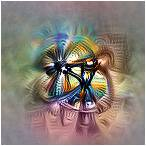
\includegraphics[scale=.5]{img134}
	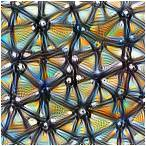
\includegraphics[scale=.5]{img138}
\end{figure}


	\begin{itemize}
		\item Feature attributions: relevant input features
	\end{itemize}
	
\begin{figure}[h]
	\centering
	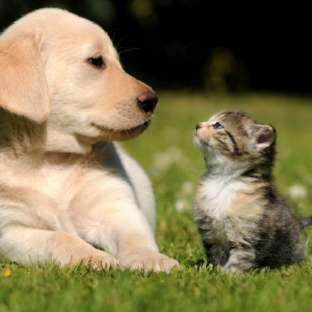
\includegraphics[scale=.5]{img145}
	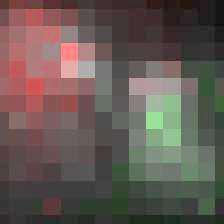
\includegraphics[scale=.5]{img149}
\end{figure}
\end{frame}

\end{document}